\subsection{MBT tests}


\subsection{Simulation results}
\subsubsection{Basic scenarios}
\begin{table}

\caption{Mean simulation results on 100 simulation runs as surrogate models on scenario \textbf{linear smooth} with sample size n = 1000 for different values of impr and alpha}
\centering \tiny
\begin{tabular}[t]{l|l|r|r|r|r|r|r|r|r|r}
\hline
black box & MBT & impr & alpha & n leaves & n leaves min & n leaves max &  $R^2_{train}$ & sd $R^2_{train}$ & $R^2_{test}$ & sd $R^2_{test}$\\
\hline
lm & SLIM & 0.15 & & 2.06 & 2 & 3 & 0.9650 & 0.0043 & 0.9631 & 0.0046\\
lm & SLIM & 0.10 & & 12.11 & 5 & 16 & 0.9965 & 0.0052 & 0.9958 & 0.0060\\
lm & SLIM & 0.05 & & 15.70 & 14 & 16 & 0.9995 & 0.0001 & 0.9993 & 0.0001\\
lm & GUIDE & 0.15 & & 2.07 & 2 & 3 & 0.9651 & 0.0044 & 0.9632 & 0.0049\\
lm & GUIDE & 0.10 & & 12.03 & 5 & 16 & 0.9965 & 0.0051 & 0.9957 & 0.0060\\
lm & GUIDE & 0.05 & & 15.75 & 14 & 16 & 0.9995 & 0.0001 & 0.9993 & 0.0001\\
lm & MOB & & 0.001 & 15.78 & 14 & 16 & 0.9994 & 0.0001 & 0.9993 & 0.0001\\
lm & MOB & & 0.010 & 15.78 & 14 & 16 & 0.9994 & 0.0001 & 0.9993 & 0.0001\\
lm & MOB & & 0.050 & 15.78 & 14 & 16 & 0.9994 & 0.0001 & 0.9993 & 0.0001\\
lm & CTree & & 0.001 & 15.22 & 13 & 17 & 0.9993 & 0.0001 & 0.9992 & 0.0001\\
lm & CTree & & 0.010 & 15.22 & 13 & 17 & 0.9993 & 0.0001 & 0.9992 & 0.0001\\
lm & CTree & & 0.050 & 15.22 & 13 & 17 & 0.9993 & 0.0001 & 0.9992 & 0.0001\\
\hline
lm &  & & & & &  & 0.9902 & 0.0006 & 0.9901 & 0.0008\\
\hline

xgboost & SLIM & 0.15 & & 2.31 & 2 & 6 & 0.9665 & 0.0069 & 0.9629 & 0.0079\\
xgboost & SLIM & 0.10 & & 7.33 & 2 & 14 & 0.9850 & 0.0060 & 0.9814 & 0.0062\\
xgboost & SLIM & 0.05 & & 14.30 & 8 & 17 & 0.9948 & 0.0010 & 0.9909 & 0.0017\\
xgboost & GUIDE & 0.15 & & 2.26 & 2 & 5 & 0.9664 & 0.0067 & 0.9628 & 0.0077\\
xgboost & GUIDE & 0.10 & & 6.92 & 2 & 14 & 0.9847 & 0.0061 & 0.9811 & 0.0062\\
xgboost & GUIDE & 0.05 & & 14.15 & 8 & 17 & 0.9945 & 0.0010 & 0.9906 & 0.0017\\
xgboost & MOB & & 0.001 & 10.89 & 8 & 13 & 0.9944 & 0.0005 & 0.9904 & 0.0011\\
xgboost & MOB & & 0.010 & 11.96 & 9 & 15 & 0.9946 & 0.0005 & 0.9906 & 0.0011\\
xgboost & MOB & & 0.050 & 12.86 & 11 & 15 & 0.9948 & 0.0005 & 0.9908 & 0.0011\\
xgboost & CTree & & 0.001 & 12.09 & 9 & 15 & 0.9940 & 0.0006 & 0.9900 & 0.0012\\
xgboost & CTree & & 0.010 & 13.21 & 10 & 15 & 0.9943 & 0.0006 & 0.9902 & 0.0013\\
xgboost & CTree & & 0.050 & 14.09 & 11 & 17 & 0.9944 & 0.0006 & 0.9904 & 0.0012\\
\hline
xgboost &  & & &  &  &  & 0.9858 & 0.0008 & 0.9768 & 0.0018\\
\hline
\end{tabular}
\label{tab:app_linear_smooth_1000}
\end{table}


\begin{figure} 
\caption{Maximum leaf size of standalone MBTs vs number of leaf nodes scenario linear smooth with $n=1000, alpha = 0.001, impr = 0.1$}
    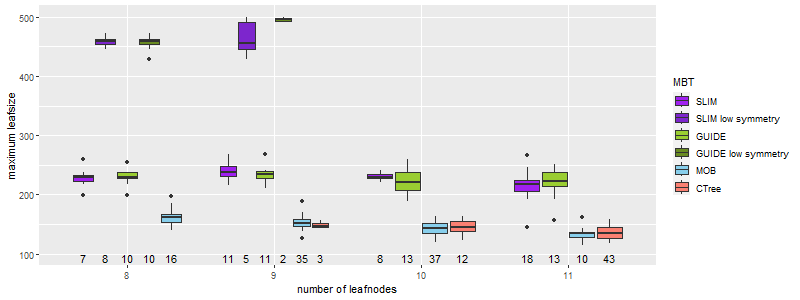
\includegraphics[width=16cm]{Figures/simulations/batchtools/basic_scenarios/linear_smooth/ls_1000_standalone_symmetrie.png}
    \label{fig:ls_1000_standalone_symmetrie}
\end{figure} 


\begin{figure} 
\caption{Test fidelity $R^2$ as surrogate on lm predictions vs number of leaf nodes scenario linear smooth with $n=1000, alpha = 0.001, impr = 0.1$}
    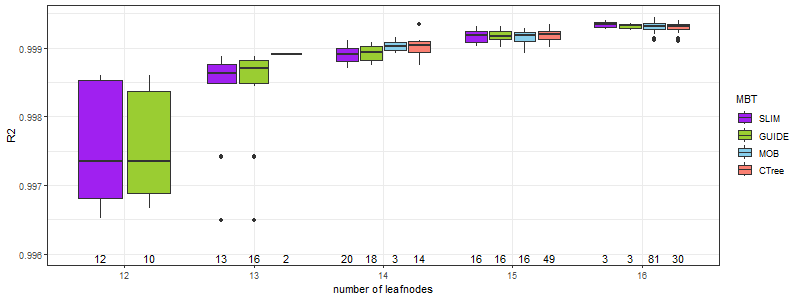
\includegraphics[width=16cm]{Figures/simulations/batchtools/basic_scenarios/linear_smooth/ls_1000_lm_r2_test.png}
    \label{fig:ls_1000_lm_r2_test}
\end{figure} 

\begin{figure} 
\caption{Test fidelity $R^2$ as surrogate on xgboost predictions vs number of leaf nodes scenario linear smooth with $n=1000, alpha = 0.001, impr = 0.1$}
    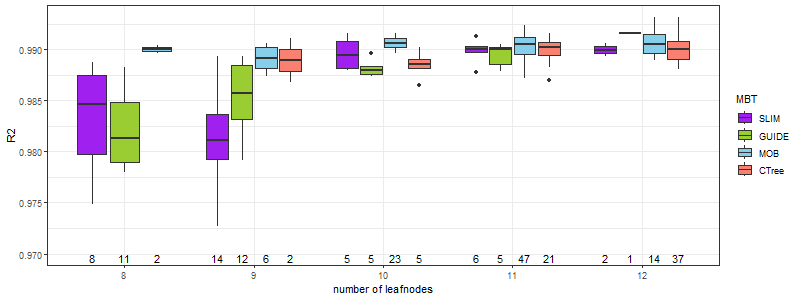
\includegraphics[width=16cm]{Figures/simulations/batchtools/basic_scenarios/linear_smooth/ls_1000_xgboost_r2_test.png}
    \label{fig:ls_1000_xgboost_r2_test}
\end{figure} 



\begin{table}

\caption{Mean simulation results on 100 simulation runs as stand alone and surrogate models on scenario \textbf{linear smooth} with sample size n = 5000 for different values of $impr$ and $alpha$}
\centering \tiny
\begin{tabular}[t]{l|l|r|r|r|r|r|r|r|r|r}
\hline
black box & MBT & impr & alpha & n leaves & n leaves min & n leaves max &  $R^2_{train}$ & sd $R^2_{train}$ & $R^2_{test}$ & sd $R^2_{test}$\\

\hline

standalone & SLIM & 0.15 & & 2.04 & 2 & 3 & 0.9542 & 0.0034 & 0.9536 & 0.0036\\
standalone & SLIM & 0.10 & & 36.94 & 15 & 58 & 0.9895 & 0.0024 & 0.9880 & 0.0024\\
standalone & SLIM & 0.05 & & 55.84 & 50 & 61 & 0.9910 & 0.0002 & 0.9890 & 0.0004\\
standalone & GUIDE & 0.15 & & 2.03 & 2 & 3 & 0.9540 & 0.0030 & 0.9534 & 0.0031\\
standalone & GUIDE & 0.10 & & 36.23 & 14 & 52 & 0.9894 & 0.0023 & 0.9881 & 0.0024\\
standalone & GUIDE & 0.05 & & 56.35 & 47 & 62 & 0.9909 & 0.0002 & 0.9891 & 0.0003\\
standalone & MOB & & 0.001 & 17.15 & 16 & 21 & 0.9901 & 0.0002 & 0.9893 & 0.0004\\
standalone & MOB & & 0.010 & 19.14 & 16 & 22 & 0.9902 & 0.0002 & 0.9894 & 0.0004\\
standalone & MOB & & 0.050 & 21.71 & 18 & 26 & 0.9903 & 0.0002 & 0.9895 & 0.0004\\
standalone & CTree & & 0.001 & 19.19 & 17 & 22 & 0.9901 & 0.0002 & 0.9894 & 0.0004\\
standalone & CTree &0 & 0.010 & 21.58 & 17 & 25 & 0.9902 & 0.0002 & 0.9895 & 0.0004\\
standalone & CTree & & 0.050 & 24.56 & 21 & 30 & 0.9903 & 0.0002 & 0.9895 & 0.0003\\


\hline
lm & SLIM & 0.15 & & 2.00 & 2 & 2 & 0.9628 & 0.0009 & 0.9625 & 0.0012\\
lm & SLIM & 0.10 & & 52.19 & 43 & 60 & 0.9999 & 0.0001 & 0.9998 & 0.0001\\
lm & SLIM & 0.05 & & 63.99 & 63 & 64 & 1.0000 & 0.0000 & 1.0000 & 0.0000\\
lm & GUIDE & 0.15 &  & 2.00 & 2 & 2 & 0.9628 & 0.0009 & 0.9625 & 0.0012\\
lm & GUIDE & 0.10 &  & 52.37 & 43 & 60 & 0.9999 & 0.0001 & 0.9998 & 0.0001\\
lm & GUIDE & 0.05 & & 63.99 & 63 & 64 & 1.0000 & 0.0000 & 1.0000 & 0.0000\\
lm & MOB & & 0.001 & 64.00 & 64 & 64 & 1.0000 & 0.0000 & 1.0000 & 0.0000\\
lm & MOB & & 0.010 & 64.00 & 64 & 64 & 1.0000 & 0.0000 & 1.0000 & 0.0000\\
lm & MOB & & 0.050 & 64.00 & 64 & 64 & 1.0000 & 0.0000 & 1.0000 & 0.0000\\
lm & CTree & & 0.001 & 63.60 & 62 & 64 & 1.0000 & 0.0000 & 1.0000 & 0.0000\\
lm & CTree & & 0.010 & 63.60 & 62 & 64 & 1.0000 & 0.0000 & 1.0000 & 0.0000\\
lm & CTree &5 & 0.050 & 63.60 & 62 & 64 & 1.0000 & 0.0000 & 1.0000 & 0.0000\\
\hline
lm & & & & & & & 0.9901 & 0.0002 & 0.9901 & 0.0003\\
\hline



xgboost & SLIM & 0.15 & & 2.22 & 2 & 7 & 0.9647 & 0.0063 & 0.9643 & 0.0063\\
xgboost & SLIM & 0.10 & & 19.23 & 3 & 40 & 0.9908 & 0.0062 & 0.9902 & 0.0062\\
xgboost & SLIM & 0.05 & & 49.05 & 34 & 56 & 0.9978 & 0.0003 & 0.9972 & 0.0003\\
xgboost & CTree & 0.15 & & 32.81 & 26 & 41 & 0.9972 & 0.0002 & 0.9965 & 0.0003\\
xgboost & CTree & 0.10 & & 36.36 & 29 & 43 & 0.9973 & 0.0002 & 0.9966 & 0.0003\\
xgboost & CTree & 0.05 & & 39.37 & 32 & 47 & 0.9974 & 0.0002 & 0.9967 & 0.0003\\
xgboost & MOB & & 0.001 & 38.44 & 29 & 47 & 0.9979 & 0.0002 & 0.9972 & 0.0003\\
xgboost & MOB & & 0.010 & 42.62 & 31 & 53 & 0.9980 & 0.0002 & 0.9973 & 0.0003\\
xgboost & MOB & & 0.050 & 46.02 & 39 & 55 & 0.9981 & 0.0002 & 0.9974 & 0.0003\\
xgboost & GUIDE & & 0.001 & 2.21 & 2 & 8 & 0.9645 & 0.0061 & 0.9641 & 0.0062\\
xgboost & GUIDE & & 0.010 & 19.27 & 3 & 38 & 0.9907 & 0.0062 & 0.9900 & 0.0062\\
xgboost & GUIDE & & 0.050 & 49.90 & 34 & 58 & 0.9977 & 0.0003 & 0.9970 & 0.0004\\
\hline
xgboost & & & & & & & 0.9877 & 0.0003 & 0.9852 & 0.0006\\
\hline

\hline
\end{tabular}
\label{tab:app_linear_smooth_5000}

\end{table}



\begin{table}

\caption{Mean simulation results on 100 simulation runs as surrogate models  on scenario \textbf{linear categorical} with sample size n = 1000 for different values of impr and alpha}
\centering \tiny
\begin{tabular}[t]{l|l|r|r|r|r|r|r|r|r|r}
\hline
black box & MBT & impr & alpha & n leaves & n leaves min & n leaves max &  $R^2_{train}$ & sd $R^2_{train}$ & $R^2_{test}$ & sd $R^2_{test}$\\
\hline
gam & SLIM & 0.15 & & 2.00 & 2 & 2 & 0.8528 & 0.0064 & 0.8513 & 0.0108\\
gam & SLIM & 0.10 & & 2.64 & 2 & 4 & 0.8972 & 0.0432 & 0.8937 & 0.0440\\
gam & SLIM & 0.05 & & 8.56 & 4 & 16 & 0.9910 & 0.0029 & 0.9893 & 0.0039\\
gam & GUIDE & 0.15 & & 2.00 & 2 & 2 & 0.8528 & 0.0064 & 0.8513 & 0.0108\\
gam & GUIDE & 0.10 & & 2.64 & 2 & 4 & 0.8972 & 0.0432 & 0.8937 & 0.0440\\
gam & GUIDE & 0.05 & & 6.06 & 4 & 13 & 0.9875 & 0.0031 & 0.9859 & 0.0038\\
gam & MOB & & 0.001 & 13.53 & 11 & 15 & 0.9773 & 0.0020 & 0.9718 & 0.0028\\
gam & MOB & & 0.010 & 14.28 & 13 & 16 & 0.9784 & 0.0020 & 0.9728 & 0.0029\\
gam & MOB & & 0.050 & 14.92 & 13 & 16 & 0.9797 & 0.0021 & 0.9740 & 0.0028\\
gam & CTree & & 0.001 & 13.89 & 11 & 16 & 0.9773 & 0.0018 & 0.9720 & 0.0028\\
gam & CTree & & 0.010 & 14.47 & 12 & 16 & 0.9779 & 0.0017 & 0.9725 & 0.0027\\
gam & CTree & & 0.050 & 14.86 & 13 & 16 & 0.9783 & 0.0016 & 0.9729 & 0.0028\\
\hline
gam & & & & & & & 0.9702 & 0.0018 & 0.9694 & 0.0029\\
\hline

xgboost & SLIM & 0.15 & & 2.00 & 2 & 2 & 0.8321 & 0.0075 & 0.8323 & 0.0118\\
xgboost & SLIM & 0.10 & & 4.00 & 4 & 4 & 0.9923 & 0.0012 & 0.9870 & 0.0029\\
xgboost & SLIM & 0.05 & & 4.00 & 4 & 4 & 0.9923 & 0.0012 & 0.9870 & 0.0029\\
xgboost & GUIDE & 0.15 & & 2.00 & 2 & 2 & 0.8321 & 0.0075 & 0.8323 & 0.0118\\
xgboost & GUIDE & 0.10 & & 4.00 & 4 & 4 & 0.9923 & 0.0012 & 0.9870 & 0.0029\\
xgboost & GUIDE & 0.05 & & 4.00 & 4 & 4 & 0.9923 & 0.0012 & 0.9870 & 0.0029\\
xgboost & MOB & & 0.001 & 13.45 & 11 & 16 & 0.9793 & 0.0063 & 0.9729 & 0.0069\\
xgboost & MOB & & 0.010 & 14.38 & 13 & 16 & 0.9831 & 0.0055 & 0.9765 & 0.0066\\
xgboost & MOB & & 0.050 & 14.63 & 13 & 16 & 0.9837 & 0.0052 & 0.9771 & 0.0062\\
xgboost & CTree & & 0.001 & 11.96 & 10 & 14 & 0.9602 & 0.0030 & 0.9545 & 0.0049\\
xgboost & CTree & & 0.010 & 12.76 & 10 & 15 & 0.9612 & 0.0033 & 0.9550 & 0.0050\\
xgboost & CTree & & 0.050 & 13.46 & 10 & 16 & 0.9623 & 0.0036 & 0.9558 & 0.0052\\
\hline
xgboost & & & & & & & 0.9876 & 0.0015 & 0.9778 & 0.0031\\
\hline
\end{tabular}
\label{tab:app_linear_abrupt_1000}

\end{table}



\begin{table}

\caption{Mean simulation results on 100 simulation runs as stand alone and surrogate models on scenario \textbf{linear categorical} with sample size n = 5000 for different values of impr and alpha}
\centering \tiny
\begin{tabular}[t]{l|l|r|r|r|r|r|r|r|r|r}
\hline
black box & MBT & impr & alpha & n leaves & n leaves min & n leaves max &  $R^2_{train}$ & sd $R^2_{train}$ & $R^2_{test}$ & sd $R^2_{test}$\\
\hline
standalone & SLIM & 0.15 & & 2.00 & 2 & 2 & 0.8277 & 0.0032 & 0.8267 & 0.0048\\
standalone & SLIM & 0.10 & & 4.00 & 4 & 4 & 0.9887 & 0.0008 & 0.9886 & 0.0011\\
standalone & SLIM & 0.05 & & 4.00 & 4 & 4 & 0.9887 & 0.0008 & 0.9886 & 0.0011\\
standalone & GUIDE & 0.15 & & 2.00 & 2 & 2 & 0.8277 & 0.0032 & 0.8267 & 0.0048\\
standalone & GUIDE & 0.10 & & 4.00 & 4 & 4 & 0.9887 & 0.0008 & 0.9886 & 0.0011\\
standalone & GUIDE & 0.05 & & 4.00 & 4 & 4 & 0.9887 & 0.0008 & 0.9886 & 0.0011\\
standalone & MOB & & 0.001 & 41.23 & 26 & 48 & 0.9896 & 0.0004 & 0.9868 & 0.0011\\
standalone & MOB & & 0.010 & 45.50 & 27 & 53 & 0.9899 & 0.0003 & 0.9871 & 0.0011\\
standalone & MOB & & 0.050 & 49.24 & 31 & 58 & 0.9902 & 0.0003 & 0.9874 & 0.0011\\
standalone & CTree & & 0.001 & 22.51 & 20 & 25 & 0.9499 & 0.0014 & 0.9462 & 0.0022\\
standalone & CTree & & 0.010 & 24.39 & 21 & 27 & 0.9502 & 0.0014 & 0.9464 & 0.0023\\
standalone & CTree & & 0.050 & 26.62 & 22 & 30 & 0.9507 & 0.0016 & 0.9468 & 0.0023\\

\hline
gam & SLIM & 0.15 & & 2.00 & 2 & 2 & 0.8532 & 0.0029 & 0.8527 & 0.0043\\
gam & SLIM & 0.10 & & 2.22 & 2 & 4 & 0.8681 & 0.0299 & 0.8668 & 0.0302\\
gam & SLIM & 0.05 & & 27.66 & 13 & 42 & 0.9940 & 0.0036 & 0.9935 & 0.0039\\
gam & GUIDE & 0.15 & & 2.00 & 2 & 2 & 0.8532 & 0.0029 & 0.8527 & 0.0043\\
gam & GUIDE & 0.10 & & 2.22 & 2 & 4 & 0.8681 & 0.0299 & 0.8668 & 0.0302\\
gam & GUIDE & 0.05 & & 14.56 & 4 & 31 & 0.9886 & 0.0038 & 0.9882 & 0.0040\\
gam & MOB & & 0.001 & 61.11 & 55 & 64 & 0.9973 & 0.0002 & 0.9966 & 0.0003\\
gam & MOB & & 0.010 & 62.42 & 59 & 64 & 0.9973 & 0.0002 & 0.9966 & 0.0002\\
gam & MOB & & 0.050 & 63.15 & 61 & 64 & 0.9974 & 0.0002 & 0.9967 & 0.0002\\
gam & CTree & & 0.001 & 33.93 & 31 & 38 & 0.9789 & 0.0007 & 0.9769 & 0.0011\\
gam & CTree & & 0.010 & 36.76 & 34 & 43 & 0.9793 & 0.0008 & 0.9772 & 0.0012\\
gam & CTree & & 0.050 & 39.43 & 36 & 45 & 0.9798 & 0.0010 & 0.9776 & 0.0013\\

\hline
gam & & & & & & & 0.9701 & 0.0010 & 0.9698 & 0.0014\\
\hline

xgboost & SLIM & 0.15 & & 2.00 & 2 & 2 & 0.8335 & 0.0033 & 0.8334 & 0.0048\\
xgboost & SLIM & 0.10 & & 4.00 & 4 & 4 & 0.9949 & 0.0009 & 0.9942 & 0.0011\\
xgboost & SLIM & 0.05 & & 4.00 & 4 & 4 & 0.9949 & 0.0009 & 0.9942 & 0.0011\\
xgboost & GUIDE & 0.15 & & 2.00 & 2 & 2 & 0.8335 & 0.0033 & 0.8334 & 0.0048\\
xgboost & GUIDE & 0.10 & & 4.00 & 4 & 4 & 0.9949 & 0.0009 & 0.9942 & 0.0011\\
xgboost & GUIDE & 0.05 & & 4.00 & 4 & 4 & 0.9949 & 0.0009 & 0.9942 & 0.0011\\
xgboost & MOB & & 0.001 & 53.91 & 49 & 60 & 0.9987 & 0.0002 & 0.9974 & 0.0007\\
xgboost & MOB & & 0.010 & 55.38 & 49 & 60 & 0.9988 & 0.0002 & 0.9974 & 0.0007\\
xgboost & MOB & & 0.050 & 56.40 & 50 & 61 & 0.9988 & 0.0002 & 0.9974 & 0.0007\\
xgboost & CTree & & 0.001 & 24.16 & 19 & 29 & 0.9600 & 0.0016 & 0.9577 & 0.0021\\
xgboost & CTree &  & 0.010 & 26.39 & 21 & 32 & 0.9605 & 0.0015 & 0.9581 & 0.0021\\
xgboost & CTree & & 0.050 & 28.97 & 22 & 36 & 0.9612 & 0.0017 & 0.9587 & 0.0023\\
\hline
xgboost & & & & & & & 0.9880 & 0.0009 & 0.9852 & 0.0009\\
\hline

\end{tabular}
\label{tab:app_linear_abrupt_5000}

\end{table}




\begin{table}

\caption{Mean simulation results on 100 simulation runs as surrogate models on scenario \textbf{linear mixed} with sample size n = 1000 for different values of impr and alpha}
\centering \tiny
\begin{tabular}[t]{l|l|r|r|r|r|r|r|r|r|r}
\hline
black box & MBT & impr & alpha & n leaves & n leaves min & n leaves max &  $R^2_{train}$ & sd $R^2_{train}$ & $R^2_{test}$ & sd $R^2_{test}$\\
\hline
lm & SLIM & 0.15 & & 3.20 & 2 & 13 & 0.8879 & 0.0309 & 0.8806 & 0.0331\\
lm & SLIM & 0.10 & & 13.07 & 5 & 16 & 0.9875 & 0.0098 & 0.9843 & 0.0108\\
lm & SLIM & 0.05 & & 14.78 & 12 & 16 & 0.9913 & 0.0020 & 0.9885 & 0.0028\\
lm & GUIDE & 0.15 & & 3.17 & 2 & 13 & 0.8872 & 0.0308 & 0.8799 & 0.0329\\
lm & GUIDE & 0.10 & & 12.66 & 7 & 16 & 0.9866 & 0.0095 & 0.9834 & 0.0106\\
lm & GUIDE & 0.05 & & 14.38 & 12 & 16 & 0.9905 & 0.0022 & 0.9876 & 0.0029\\
lm & MOB & & 0.001 & 14.99 & 13 & 17 & 0.9882 & 0.0016 & 0.9838 & 0.0021\\
lm & MOB & & 0.010 & 14.99 & 13 & 17 & 0.9882 & 0.0016 & 0.9838 & 0.0021\\
lm & MOB & & 0.050 & 14.99 & 13 & 17 & 0.9882 & 0.0016 & 0.9838 & 0.0021\\
lm & CTree & & 0.001 & 15.05 & 13 & 17 & 0.9880 & 0.0016 & 0.9841 & 0.0019\\
lm & CTree & & 0.010 & 15.05 & 13 & 17 & 0.9880 & 0.0016 & 0.9841 & 0.0019\\
lm & CTree & & 0.050 & 15.05 & 13 & 17 & 0.9880 & 0.0016 & 0.9841 & 0.0019\\

\hline
lm & & & & & & & 0.9902 & 0.0006 & 0.9898 & 0.0008\\
\hline


xgboost & SLIM & 0.15 & & 4.47 & 2 & 13 & 0.9067 & 0.0336 & 0.9013 & 0.0339\\
xgboost & SLIM & 0.10 & & 12.80 & 7 & 16 & 0.9832 & 0.0089 & 0.9724 & 0.0103\\
xgboost & SLIM & 0.05 & & 14.80 & 12 & 17 & 0.9870 & 0.0018 & 0.9764 & 0.0044\\
xgboost & GUIDE & 0.15 & & 4.37 & 2 & 13 & 0.9059 & 0.0335 & 0.9005 & 0.0339\\
xgboost & GUIDE & 0.10 & & 12.48 & 6 & 16 & 0.9822 & 0.0098 & 0.9715 & 0.0112\\
xgboost & GUIDE & 0.05 & & 14.47 & 12 & 17 & 0.9863 & 0.0022 & 0.9758 & 0.0047\\
xgboost & MOB & & 0.001 & 14.82 & 13 & 17 & 0.9853 & 0.0018 & 0.9745 & 0.0047\\
xgboost & MOB & & 0.010 & 14.94 & 13 & 17 & 0.9854 & 0.0017 & 0.9746 & 0.0046\\
xgboost & MOB & & 0.050 & 14.94 & 13 & 17 & 0.9854 & 0.0017 & 0.9746 & 0.0046\\
xgboost & CTree & & 0.001 & 15.03 & 13 & 17 & 0.9850 & 0.0017 & 0.9743 & 0.0042\\
xgboost & CTree & & 0.010 & 15.07 & 13 & 17 & 0.9850 & 0.0017 & 0.9743 & 0.0042\\
xgboost & CTree & & 0.050 & 15.07 & 13 & 17 & 0.9850 & 0.0017 & 0.9743 & 0.0042\\
\hline
xgboost & & & & & & & 0.9859 & 0.0014 & 0.9682 & 0.0042\\
\hline
\end{tabular}
\label{tab:app_linear_mixed_1000}

\end{table}





\begin{table}

\caption{Mean simulation results on 100 simulation runs as stand alone and surrogate models on scenario \textbf{linear mixed} with sample size n = 5000 for different values of impr and alpha}
\centering \tiny
\begin{tabular}[t]{l|l|r|r|r|r|r|r|r|r|r}
\hline
black box & MBT & impr & alpha & n leaves & n leaves min & n leaves max &  $R^2_{train}$ & sd $R^2_{train}$ & $R^2_{test}$ & sd $R^2_{test}$\\
\hline
standalone & SLIM & 0.15 & & 2.30 & 2 & 8 & 0.8637 & 0.0165 & 0.8626 & 0.0176\\
standalone & SLIM & 0.10 & & 38.96 & 21 & 54 & 0.9865 & 0.0029 & 0.9849 & 0.0030\\
standalone & SLIM & 0.05 & & 59.03 & 51 & 64 & 0.9904 & 0.0005 & 0.9884 & 0.0006\\
standalone & GUIDE & 0.15 & & 2.30 & 2 & 8 & 0.8637 & 0.0165 & 0.8626 & 0.0176\\
standalone & GUIDE & 0.10 & & 38.06 & 21 & 54 & 0.9866 & 0.0028 & 0.9851 & 0.0029\\
standalone & GUIDE & 0.05 & & 58.20 & 45 & 63 & 0.9903 & 0.0005 & 0.9885 & 0.0006\\
standalone & MOB & & 0.001 & 48.54 & 43 & 55 & 0.9888 & 0.0004 & 0.9861 & 0.0007\\
standalone & MOB & & 0.010 & 53.17 & 48 & 58 & 0.9891 & 0.0003 & 0.9864 & 0.0007\\
standalone & MOB & & 0.050 & 56.07 & 51 & 60 & 0.9893 & 0.0003 & 0.9866 & 0.0006\\
standalone & CTree & & 0.001 & 51.70 & 47 & 57 & 0.9887 & 0.0004 & 0.9858 & 0.0006\\
standalone & CTree & & 0.010 & 54.85 & 50 & 58 & 0.9889 & 0.0004 & 0.9860 & 0.0006\\
standalone & CTree & & 0.050 & 56.76 & 52 & 61 & 0.9890 & 0.0003 & 0.9860 & 0.0006\\

\hline
lm & SLIM & 0.15 & & 2.17 & 2 & 16 & 0.8683 & 0.0094 & 0.8677 & 0.0103\\
lm & SLIM & 0.10 & & 39.69 & 19 & 55 & 0.9956 & 0.0028 & 0.9953 & 0.0030\\
lm & SLIM & 0.05 & & 57.51 & 46 & 64 & 0.9991 & 0.0005 & 0.9990 & 0.0006\\
lm & GUIDE & 0.15 & & 2.17 & 2 & 16 & 0.8683 & 0.0094 & 0.8677 & 0.0103\\
lm & GUIDE & 0.10 & & 40.32 & 19 & 55 & 0.9960 & 0.0026 & 0.9956 & 0.0028\\
lm & GUIDE & 0.05 & & 57.32 & 46 & 64 & 0.9991 & 0.0005 & 0.9990 & 0.0006\\
lm & MOB & & 0.001 & 63.11 & 60 & 64 & 0.9973 & 0.0002 & 0.9964 & 0.0003\\
lm & MOB & & 0.010 & 63.11 & 60 & 64 & 0.9973 & 0.0002 & 0.9964 & 0.0003\\
lm & MOB & & 0.050 & 63.11 & 60 & 64 & 0.9973 & 0.0002 & 0.9964 & 0.0003\\
lm & CTree & & 0.001 & 62.72 & 59 & 64 & 0.9973 & 0.0002 & 0.9964 & 0.0003\\
lm & CTree & & 0.010 & 62.72 & 59 & 64 & 0.9973 & 0.0002 & 0.9964 & 0.0003\\
lm & CTree & & 0.050 & 62.72 & 59 & 64 & 0.9973 & 0.0002 & 0.9964 & 0.0003\\
\hline
lm & & & & & & & 0.9901 & 0.0003 & 0.9902 & 0.0004\\
\hline


\hline
xgboost & SLIM & 0.15 & & 2.22 & 2 & 12 & 0.8693 & 0.0121 & 0.8706 & 0.0129\\
xgboost & SLIM & 0.10 & & 39.52 & 23 & 53 & 0.9931 & 0.0027 & 0.9914 & 0.0027\\
xgboost & SLIM & 0.05 & & 56.86 & 46 & 63 & 0.9964 & 0.0005 & 0.9948 & 0.0007\\
xgboost & GUIDE & 0.15 & & 2.15 & 2 & 9 & 0.8693 & 0.0119 & 0.8705 & 0.0127\\
xgboost & GUIDE & 0.10 & & 38.13 & 22 & 52 & 0.9928 & 0.0027 & 0.9912 & 0.0028\\
xgboost & GUIDE & 0.05 & & 56.72 & 46 & 63 & 0.9963 & 0.0006 & 0.9946 & 0.0007\\
xgboost & MOB & & 0.001 & 58.76 & 54 & 63 & 0.9961 & 0.0003 & 0.9942 & 0.0005\\
xgboost & MOB & & 0.010 & 59.47 & 55 & 64 & 0.9961 & 0.0003 & 0.9943 & 0.0005\\
xgboost & MOB & & 0.050 & 59.69 & 55 & 64 & 0.9961 & 0.0003 & 0.9943 & 0.0005\\
xgboost & CTree & & 0.001 & 58.51 & 53 & 62 & 0.9956 & 0.0003 & 0.9936 & 0.0005\\
xgboost & CTree & & 0.010 & 58.95 & 54 & 63 & 0.9956 & 0.0003 & 0.9936 & 0.0005\\
xgboost & CTree & & 0.050 & 59.09 & 54 & 63 & 0.9956 & 0.0003 & 0.9936 & 0.0005\\
\hline
xgboost & & & & & & & 0.9877 & 0.0007 & 0.9836 & 0.0011\\
\hline

\end{tabular}
\label{tab:app_linear_mixed_5000}

\end{table}



\subsubsection{Correlated features}

\subsubsection{Big number of noise features}

\subsubsection{Nonlinear mixed}


\subsubsection{Selection Bias}